\documentclass[../main.tex]{subfiles}

\begin{document}
\chapter{理科生玩转Python}\label{chap:python-advanced}
\begin{flushright}
    \emph{这里默认你已经会Python的基本语法了,如果不会,请先阅读《Python高速入门》一节!}
\end{flushright}

Python作为时下最流行的高级脚本语言之一,在多个领域有着广泛的应用;不仅是文科学生可以利用它来进行数据分析、自然语言处理等工作,理科生也可以利用它来进行科学计算、机器学习等任务。本章将介绍Python的一些非常常用的包(理工科常用),涵盖了机器学习、数学建模、数值计算、信号处理、算法可视化等大量内容,供大家按需使用。

\section{PyTorch:让你的电脑会学习}
\begin{flushright}
    \emph{建议本节阅读者有一定的线性代数基础。}
\end{flushright}

PyTorch是一个开源的机器学习框架,广泛应用于科研领域,和大名鼎鼎的TensorFlow齐名。由于PyTorch更加灵活、动态,因此在学生和科研人员中更受欢迎;而TensorFlow则因为性能更强大而多用于生产环境。当然,我们在这里不讨论后者(因为我也不大会用)。

即使不用它来做机器学习,PyTorch也可以作为一个非常强大的数值计算库来使用,例如从一大堆点中拟合出一条直线等。或者说,Numpy++。

\subsection{安装}

如果希望使用PyTorch,一般建议先有一个Python虚拟环境和一个显卡(最好是英伟达)。如果没有显卡,PyTorch也可以在CPU上运行,但速度会慢很多。

首先在终端中运行这个命令,来判断你的显卡是什么CUDA版本:
\begin{lstlisting}[language=bash]
nvidia-smi
\end{lstlisting}

然后去\href{https://pytorch.org/get-started/locally/}{PyTorch官网},根据你的CUDA版本和系统环境选择合适的安装命令。(无GPU版本则选CPU。)

安装完毕后,使用以下命令来测试PyTorch是否安装成功:
\begin{lstlisting}[language=python]
python -c "import torch, torch.cuda; print(torch.__version__, torch.cuda.is_available())"
\end{lstlisting}
要是输出True,说明你的GPU准备好了。即使是没有GPU的电脑,PyTorch也可以正常运行,只是速度会慢很多。

\subsection{张量、梯度下降和自动求导}

刚刚说到,PyTorch是一个机器学习库,因此我们至少应当了解这些基本概念。

张量(Tensor)是PyTorch的核心数据结构,类似于Numpy中的数组。张量可以是标量(0维)、向量(1维)、矩阵(2维)或更高维度的数组。使用PyTorch的情况下,张量可以在CPU或GPU上运行,显著提高并行速度。

梯度(Gradient)可以通俗理解为“导数”,在机器学习上特指损失函数相对于模型参数的导数,表示损失函数在某一点的变化率。而梯度下降则指,通过计算损失函数相对于模型参数的梯度来更新模型参数,使得损失函数最小化。PyTorch提供了自动求导功能,可以自动计算梯度。自动求导则是指,PyTorch可以自动计算张量的梯度,这样我们就不需要手动计算导数了。

\begin{lstlisting}
import torch

# 像 NumPy 一样造张量
x = torch.arange(12, dtype=torch.float32).reshape(3, 4)
y = torch.randn_like(x)
z = torch.tensor([1., 2., 3.], dtype=torch.float32, requires_grad=True)  # requires_grad=True表示需要计算梯度

# 一句话把张量搬到GPU上
if torch.cuda.is_available(): # 如果确定GPU可用,这个可以不写
    x = x.cuda()
    y = y.cuda()

# 广播、切片、点乘,全部 NumPy 语法
xy = (x @ y.T).relu()          # relu 也能直接点出来

z2 = x.pow(2).sum()  # 求平方和
z2.backward()  # 自动求导,计算 z2 相对于 x 的梯度
print(x.grad)  # 输出 x 的梯度,输出应当是[2., 4., 6.]

\end{lstlisting}

上文中的\texttt{x\@ y.T}的意思是矩阵乘法(点乘),\texttt{y.T}表示\texttt{y}的转置。PyTorch的张量支持广播(Broadcasting)机制,这意味着当两个张量的形状不同时,PyTorch会自动调整它们的形状以进行运算。relu是一个函数,用于将负值变为0,非负值不变。

\subsection{数据集、数据加载器、预处理}

在机器学习中,我们通常需要处理大量的数据。PyTorch提供了数据集(Dataset)和数据加载器(DataLoader)来帮助我们处理数据,而不是使用for循环来缓慢地加载数据。

\begin{lstlisting}
    from torch.utils.data import Dataset, DataLoader
from torchvision import datasets, transforms

transform = transforms.Compose([    # 数据预处理
    transforms.ToTensor(),                    # HWC to CHW, [0,255] → [0,1]
    transforms.Normalize((0.1307,), (0.3081,)) # 数据集统计均值方差
])

train_ds = datasets.MNIST(root='.', train=True,  download=True, transform=transform)
train_dl = DataLoader(train_ds, batch_size=256, shuffle=True, num_workers=4)

for x, y in train_dl:        # x.shape == [256, 1, 28, 28]
    ... # 这里应当存在一些代码用于表示训练逻辑,但是这里懒得写了
\end{lstlisting}

\subsection{\texttt{nn.Module}搭积木式写网络}

PyTorch的\texttt{nn.Module}是一个非常强大的模块化网络构建工具。我们可以通过继承\texttt{nn.Module}来定义自己的网络结构。例如:

\begin{lstlisting}
    import torch.nn as nn

class MLP(nn.Module):
    def __init__(self):
        super().__init__()
        self.net = nn.Sequential(
            nn.Flatten(),
            nn.Linear(28*28, 256),
            nn.ReLU(),
            nn.Linear(256, 10)
        )

    def forward(self, x):
        return self.net(x)

model = MLP().cuda() if torch.cuda.is_available() else MLP()
\end{lstlisting}

上述代码定义了一个叫做MLP的多层感知机(MLP)模型\footnote{MLP是最基础的神经网络结构之一,适用于处理结构化数据,如图像、文本等。}。它包含了一个输入层、一个隐藏层和一个输出层。我们使用\texttt{nn.Flatten}将输入的28x28的图像展平为一维向量,然后通过两个全连接层(\texttt{nn.Linear})进行处理,中间使用ReLU激活函数(\texttt{nn.ReLU})来增加非线性。

在上述实践中,我们使用\texttt{nn.Sequential}来将多个层按顺序组合起来,并使用\texttt{nn.Module}的\texttt{forward}方法定义了前向传播的逻辑。

\subsection{真正训练}

这里的内容实际上应该是科研组干的或者上课讲的。我们在这里举个例子就好了!

\begin{lstlisting}
opt = torch.optim.Adam(model.parameters(), lr=1e-3)
loss_fn = nn.CrossEntropyLoss()

for epoch in range(3):
    for x, y in train_dl:
        x, y = x.cuda(), y.cuda()
        pred = model(x)
        loss = loss_fn(pred, y)

        opt.zero_grad()
        loss.backward()
        opt.step()

    print(f"epoch {epoch}: loss={loss.item():.4f}")
\end{lstlisting}

上述代码展示了一个简单的训练循环。我们使用Adam优化器(\texttt{torch.optim.Adam})来更新模型参数,使用交叉熵损失函数(\texttt{nn.CrossEntropyLoss})来计算损失。每个epoch中,我们遍历数据加载器(\texttt{train\_dl}),获取输入数据和标签,然后进行前向传播、计算损失、反向传播和参数更新。

\subsection{做个实验}

多说无益。我们来做个实验,看看PyTorch能不能学会识别手写数字。

MNIST数据集是一个经典的手写数字识别数据集,包含了60000个训练样本和10000个测试样本。我们可以使用PyTorch来加载这个数据集,并训练一个简单的神经网络来进行手写数字识别。当然,想让啥也不会的同学们写个代码帮助计算机识别0到9的数字还是太难了,我们就写个鉴别0和1的二分类器吧。

\begin{lstlisting}
#!/usr/bin/env python3 # 这是一个shebang行,不写也行
"""
mnist_01_linear.py
用 PyTorch 线性分类器区分 MNIST 的 0 和 1
运行环境: Python最低3.8, PyTorch最低1.13, torchvision
"""

import torch
import torch.nn as nn
from torch.utils.data import DataLoader, Subset
from torchvision import datasets, transforms
from sklearn.metrics import accuracy_score   # 仅用来算准确率,可省

# 1. 超参数,用于提纲挈领地控制训练流程
DEVICE = 'cuda' if torch.cuda.is_available() else 'cpu'
BATCH_SIZE = 256    # 批大小,即每次训练使用多少张图片
EPOCHS = 5          # 训练轮数
LR = 0.1            # 学习率,控制参数更新的步长

# 2. 只保留 0 和 1 的子数据集,别的全都不要
transform = transforms.ToTensor()   # 0-255 -> 0-1, [1,28,28]

def get_binary_mnist(root='.', train=True):
    full = datasets.MNIST(root=root, train=train, download=True, transform=transform)
    idx = (full.targets == 0) | (full.targets == 1)
    return Subset(full, torch.where(idx)[0])

train_ds = get_binary_mnist(train=True)
test_ds  = get_binary_mnist(train=False)

train_dl = DataLoader(train_ds, batch_size=BATCH_SIZE, shuffle=True)
test_dl  = DataLoader(test_ds,  batch_size=BATCH_SIZE)

# 3. 线性二分类器
class LogisticRegression(nn.Module):
    def __init__(self):
        super().__init__()
        self.flatten = nn.Flatten()           # 1*28*28 -> 784
        self.linear  = nn.Linear(28*28, 1)    # 输出 1 个 logit

    def forward(self, x):
        x = self.flatten(x)
        return self.linear(x).squeeze()       # [B,1] -> [B]

model = LogisticRegression().to(DEVICE)

# 4. 损失 & 优化
criterion = nn.BCEWithLogitsLoss()            # 自带 sigmoid
optimizer = torch.optim.SGD(model.parameters(), lr=LR) # 使用最简单的 SGD 优化器

# 5. 训练
for epoch in range(1, EPOCHS+1):
    model.train()
    for x, y in train_dl:
        x, y = x.to(DEVICE), y.float().to(DEVICE)  
        optimizer.zero_grad()
        logits = model(x)
        loss = criterion(logits, y)
        loss.backward()
        optimizer.step()
    print(f"Epoch {epoch}: loss={loss.item():.4f}")

# 6. 测试 
model.eval()
all_pred, all_true = [], []
with torch.no_grad():
    for x, y in test_dl:
        x = x.to(DEVICE)
        probs = torch.sigmoid(model(x))
        preds = (probs > 0.5).long()
        all_pred.append(preds.cpu())
        all_true.append(y)

# 7. 计算准确率
all_pred = torch.cat(all_pred).numpy()
all_true = torch.cat(all_true).numpy()
print("Test accuracy:", accuracy_score(all_true, all_pred))
\end{lstlisting}

以上代码使用的是784 to 1的线性分类器(Logistic Regression),通过sigmoid函数将输出转换为概率。我们使用二元交叉熵损失函数(\texttt{nn.BCEWithLogitsLoss})来计算损失,并使用随机梯度下降(SGD)优化器来更新模型参数。

同学们很可能看不懂这些代码的细节,顶多能知道每一块代码是做什么的。不过,没关系!只要理解了整体用法,剩下的就是逐步掌握细节;而这则需要同学们在之后的课程和学习中不断探索和实践,不断优化自己的模型、调整模型的参数,从而真正成为机器学习的高手。

\subsection{我看完了,然后呢}

看完本节内容估计只需要五分钟。既然同学们这么快就看完了我写的基础内容,那么接下来就可以去官网自己查自己需要的内容了。PyTorch官方的\href{https://docs.pytorch.org/tutorials/beginner/deep_learning_60min_blitz.html}{60分钟速通PyTorch}课程链接我已经放在这里了,感兴趣的同学们可以自己去看看。

\section{Numpy+Scipy:科学计算的利器}

\begin{flushright}
    \emph{建议本节阅读者有一定的线性代数和高等数学基础。}
\end{flushright}

Numpy和Scipy是Python中用于科学计算的两个重要库。Numpy提供了高效的多维数组对象和各种数学函数,而Scipy则在此基础上提供了更多的科学计算功能,如优化、积分、插值等。掌握了这两个库,Python就具有了MatLab的核心战斗力,却又保留了Python的灵活性和易用性。

\subsection{Numpy:多维数组和矩阵运算}

Numpy的核心数据类型是ndarray(N维数组),它可以存储多维数据。这玩意可不是低级的“列表+语法糖”,而是一个真正的C风格连续内存块和元数据。它要求我们应当具有\textbf{向量思维}。

对于该数据类型,我们熟悉这两个术语就可以:形状(shape)和步长(stride)。形状表示数组的维度;步长表示每个维度的跨度。
举例:
\begin{lstlisting}
import numpy as np
a = np.arange(12).reshape(3, 4)
a.strides        # 每一行 32 字节,因为 int64=8B * 4 列

# 应当是(32, 8)
\end{lstlisting}

\subsubsection{向量化三件套}

Numpy的向量化三件套是指:广播(Broadcasting)、通用函数(ufuncs)和切片视图(Slicing Views)。这三者结合起来,可以让我们在处理大规模数据时,避免使用for循环,从而提高计算效率。

一个个讲吧:
\begin{itemize}
    \item 广播:从尾部维度开始比较,长度相等或其中一维为 1 即可兼容。
    \begin{lstlisting}
pts = np.random.randn(1000, 3)
t   = np.array([1.0, 2.0, 3.0])
shifted = pts + t       # (1000,3) + (3,),自动广播
    \end{lstlisting}
    \item 通用函数:Numpy提供了许多通用函数(ufuncs),可以对数组进行元素级的操作,如加减乘除、三角函数等。
    \begin{lstlisting}
pts = np.random.randn(1000, 3)
norms = np.linalg.norm(pts, axis=1)  # 计算每个点的范数
\end{lstlisting}
    \item 切片视图:Numpy的切片操作返回的是原数组的视图,而不是复制数据。这意味着对切片的修改会影响原数组。
    \begin{lstlisting}
pts = np.random.randn(1000, 3)
pts[:, 0] = 0.0  # 将所有点的 x 坐标设为 0
print(pts[0])  # 输出第一个点的坐标,x 坐标应为 0.0
    \end{lstlisting}
\end{itemize}

不如做个性能对比实验:给你一千万(1e7)个点,计算它们的欧氏范数。欧式范数的计算方法是:$\sqrt{x^2 + y^2 + z^2}$。vanilla写法自己去写,我这里只给出Numpy的写法:
\begin{lstlisting}
import numpy as np
pts = np.random.randn(int(1e7), 3)  # 生成一千万个三维点
norms = np.sqrt(np.einsum('ij,ij->i', pts, pts))  # 使用爱因斯坦求和约定计算欧氏范数
\end{lstlisting}
运行你的代码和Numpy的代码,比较一下性能。使用爱因斯坦求和约定计算范数应当是最快的算法,预计比基准线快50倍以上。

\subsection{Scipy:科学计算的扩展}

Scipy是站在Numpy上的科学计算库,提供了更多的科学计算功能,如优化、插值、积分、信号处理等。Scipy的模块化设计使得它可以非常方便地进行各种科学计算,可以将高阶算法压成一行随便用,显著加快了运算效率。

\subsubsection{优化}
Scipy提供了许多优化算法,可以用于许多问题,例如梯度下降、牛顿法、共轭梯度等。我们可以使用\texttt{scipy.optimize}模块来进行优化,以下函数是一个最小化函数的例子:
\begin{lstlisting}
from scipy.optimize import minimize

rosenbrock = lambda x: (1-x[0])**2 + 100*(x[1]-x[0]**2)**2
result = minimize(rosenbrock, x0=[2,2], method='BFGS', jac='2-point')
print(result.x, result.nit)   # [1. 1.] 24
\end{lstlisting}
以上代码使用BFGS算法最小化Rosenbrock函数,初始点为(2, 2),最终结果应当接近(1, 1)。不知道Rosenbrock函数是什么的同学可以看\href{https://en.wikipedia.org/wiki/Rosenbrock_function}{维基百科}。

比较常见的minimize优化参数包括jac(梯度计算方式)、tol(容忍度)、options(其他选项)等。Scipy还提供了许多其他的优化函数,如\texttt{scipy.optimize.linprog}用于线性规划,\texttt{scipy.optimize.curve\_fit}用于曲线拟合等。这些函数同学们都可以查阅\href{https://docs.scipy.org/doc/scipy/reference/optimize.html}{Scipy官方文档}。

\subsubsection{稀疏矩阵}

稀疏矩阵指的是大多数元素是0的矩阵,在科学计算中非常常见。Scipy提供了\texttt{scipy.sparse}模块来处理稀疏矩阵。

\begin{lstlisting}[language=python]
from scipy.sparse import diags
n = 1000
k = [-1, 0, 1]
data = [np.full(n-1, -1), np.full(n, 2), np.full(n-1, -1)]
L = diags(data, k, shape=(n, n), format='csr')  # 三对角稀疏

from scipy.sparse.linalg import spsolve
x = spsolve(L, np.ones(n))  # 求解 Lx = 1
\end{lstlisting}
以上代码创建了一个三对角稀疏矩阵L,主对角线为2,次对角线为-1。Scipy的稀疏矩阵支持许多操作,如矩阵乘法、求逆等。例如上述元素代码中使用\texttt{spsolve}函数来求解线性方程组$Lx = 1$,其中$1$是一个全1向量。

\subsubsection{数值积分}

有些时候,对于一些积分我们不是很容易求出解析解,这时候就需要数值积分了。Scipy提供了\texttt{scipy.integrate}模块来进行数值积分。
\begin{lstlisting}[language=python]
from scipy.integrate import quad
val, abserr = quad(lambda x: np.exp(-x**2), 0, np.inf)
print(np.sqrt(np.pi)/2 - val)  # 输出误差, ~1e-13
\end{lstlisting}
上述代码使用\texttt{quad}函数计算了从0到无穷大的高斯函数的积分,结果应当接近$\sqrt{\pi}/2$。\texttt{quad}函数返回两个值:积分值和绝对误差。

\subsection{两个一起,双倍开心}

一般情况下,我们需要将Numpy和Scipy协同使用以实现更强大的功能,前者向量化批处理,后者提供算法和工具,十分快乐。以下是一个示例,利用二次Bezier曲线拟合100个带噪声的二维点,并最小化点到曲线距离的平方和:
\begin{lstlisting}[language=python]
import numpy as np
from scipy.optimize import minimize

# 数据
pts = np.c_[np.linspace(0,1,100)**2,
            np.linspace(0,1,100)] + np.random.randn(100,2)*0.02

# Bezier 曲线函数
bezier = lambda t, p0, p1, p2: (1-t)**2*p0 + 2*(1-t)*t*p1 + t**2*p2

def error(params):
    p0, p1, p2 = params.reshape(3,2)
    t = np.linspace(0,1,100)
    curve = bezier(t[:,None], p0, p1, p2)
    return np.sum((curve - pts)**2)

result = minimize(error, x0=np.random.rand(6))
print(result.x.reshape(3,2))
\end{lstlisting}
上述代码首先生成了100个带噪声的二维点,然后定义了一个二次Bezier曲线函数,并使用最小化算法拟合这些点。最终输出的结果是拟合曲线的控制点坐标。

\section{Matplotlib:数据可视化的神器}

在上一章中我们讲过,可以使用Matplotlib来绘制各种统计图表和数据可视化图形。这是Python里面最常用的可视化库之一,也是生态中最早、最稳定、最通用的可视化库。另一方面,它能够和Numpy、Pandas等库无缝集成,提供了强大的绘图功能。

\subsection{基本用法}

Matplotlib的基本用法是通过pyplot模块来实现的。我们可以使用以下代码来绘制一个简单的折线图:
\begin{lstlisting}[language=python]
import matplotlib.pyplot as plt
import numpy as np

x = np.linspace(0, 10, 100)
y = np.sin(x)

plt.plot(x, y, label='sin(x)')  # 绘制曲线
plt.xlabel('x')  # 添加坐标轴标签
plt.ylabel('sin(x)')  # 添加坐标轴标签
plt.title('Simple Plot')  # 添加标题
plt.legend()  # 添加图例
plt.show()  # 显示图形
\end{lstlisting}
上述代码使用\texttt{plt.plot}函数绘制了一个简单的折线图,并添加了坐标轴标签、标题和图例。最后使用\texttt{plt.show()}函数显示图形。

\begin{figure}[htbp]
    \centering
    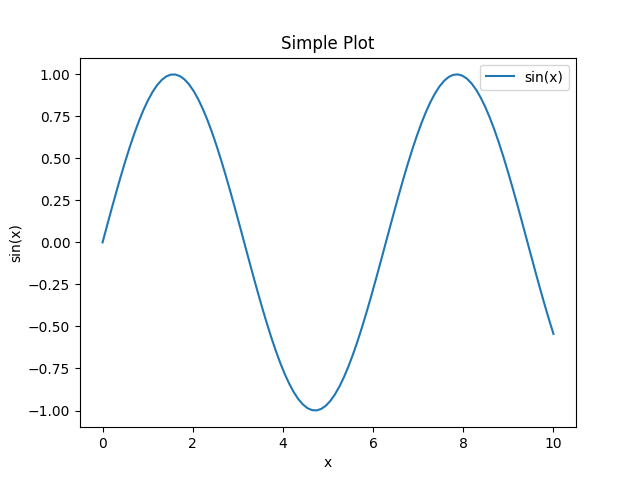
\includegraphics[width=0.8\textwidth]{images/plt/Figure_1.png}
\end{figure}

除了使用简洁的\texttt{pyplot}以外,还可以使用面向对象风格的API来绘图,便于封装和复用:

\begin{lstlisting}
import matplotlib.pyplot as plt
import numpy as np

x = np.linspace(0, 2*np.pi, 100)  # Create x values from 0 to 2pi

fig, ax = plt.subplots(figsize=(8, 6))  # 创建一个图形和坐标轴对象
ax.plot(x, np.sin(x), label=r'$sin(x)$', color='tab:blue', lw=2)  # 绘制曲线
ax.plot(x, np.cos(x), label=r'$cos(x)$', ls='--')  # 绘制曲线
ax.set_xlabel(r'$x$')  # 添加坐标轴标签
ax.set_ylabel(r'$y$')  # 添加坐标轴标签
ax.legend()  # 添加图例
ax.set_title('Matplotlib Example')  # 添加标题
fig.tight_layout()  # 自动调整布局
plt.show()  # 显示图形
\end{lstlisting}
上述代码使用\texttt{plt.subplots}函数创建了一个图形和坐标轴对象,然后使用坐标轴对象的\texttt{plot}方法绘制曲线。这样可以更灵活地控制图形的各个部分。

\begin{figure}[htbp]
    \centering
    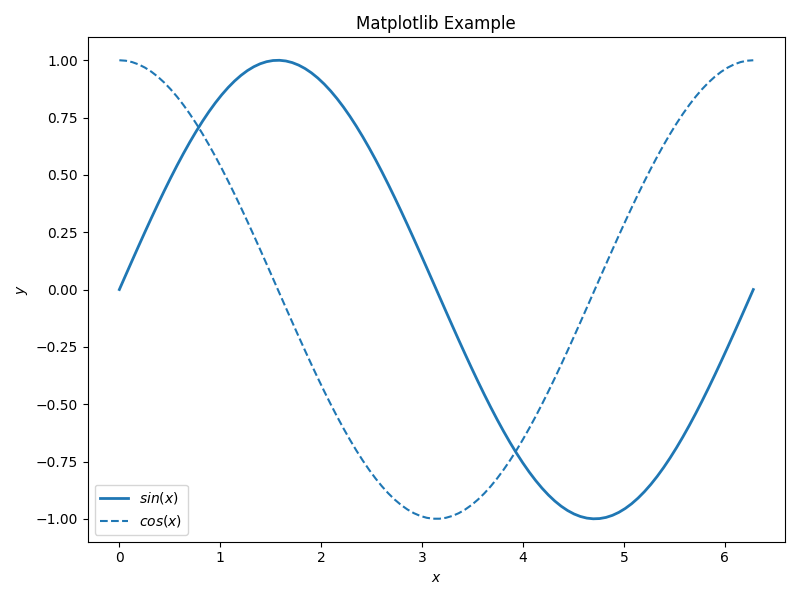
\includegraphics[width=0.8\textwidth]{images/plt/Figure_2.png}
\end{figure}

\subsection{和其他包协同工作}

Matplotlib可以和Numpy、Pandas等库无缝集成,提供了强大的绘图功能。例如,我们可以使用Numpy生成数据,然后使用Matplotlib绘制图形:
\begin{lstlisting}
import matplotlib.pyplot as plt
import numpy as np

X, Y = np.meshgrid(np.linspace(-3, 3, 300),
                   np.linspace(-3, 3, 300))
Z = np.sinc(np.sqrt(X**2 + Y**2))

fig, ax = plt.subplots()
c = ax.contourf(X, Y, Z, levels=50, cmap='viridis')
fig.colorbar(c, ax=ax)

plt.title('Contour Plot of Sinc Function')
plt.xlabel('X-axis')
plt.ylabel('Y-axis')
plt.show()
\end{lstlisting}

\begin{figure}
    \centering
    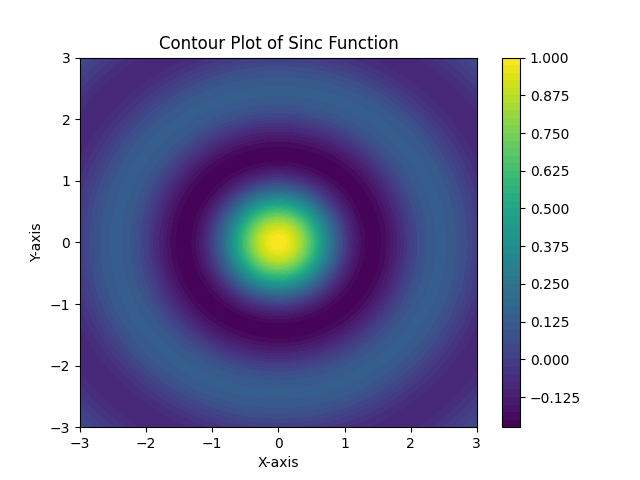
\includegraphics[width=0.8\textwidth]{images/plt/Figure_3.png}
\end{figure}

或者使用Pandas绘制数据框的图形:
\begin{lstlisting}
import pandas as pd

df = pd.read_csv('experiment.csv')
ax = df.plot(x='voltage', y='current', kind='scatter', color='k')
ax.set_xlabel('Voltage (V)')
ax.set_ylabel('Current (mA)')
# 这只是一个示例,没有数据是真不行,后面绘图的逻辑自己写就好了
\end{lstlisting}

\subsection{子图布局}

在实际应用中,我们经常需要将多个图形绘制在同一个窗口中,这就需要用到子图的概念。Matplotlib提供了\texttt{subplot}和\texttt{subplots}函数来创建子图。

\begin{lstlisting}[language=python]
import matplotlib.pyplot as plt
import numpy as np

x = np.linspace(0, 10, 100)
y1 = np.sin(x)
y2 = np.cos(x)

fig, axs = plt.subplots(2, 1, figsize=(8, 6))  # 创建2行1列的子图
axs[0].plot(x, y1, label='sin(x)', color='tab:blue')
axs[0].set_title('Sine Function')
axs[1].plot(x, y2, label='cos(x)', color='tab:orange')
axs[1].set_title('Cosine Function')
plt.tight_layout()
plt.show()
\end{lstlisting}
上述代码创建了一个包含两个子图的图形窗口,分别绘制了正弦函数和余弦函数。使用\texttt{plt.tight\_layout()}函数可以自动调整子图之间的间距。

\begin{figure}[htbp]
    \centering
    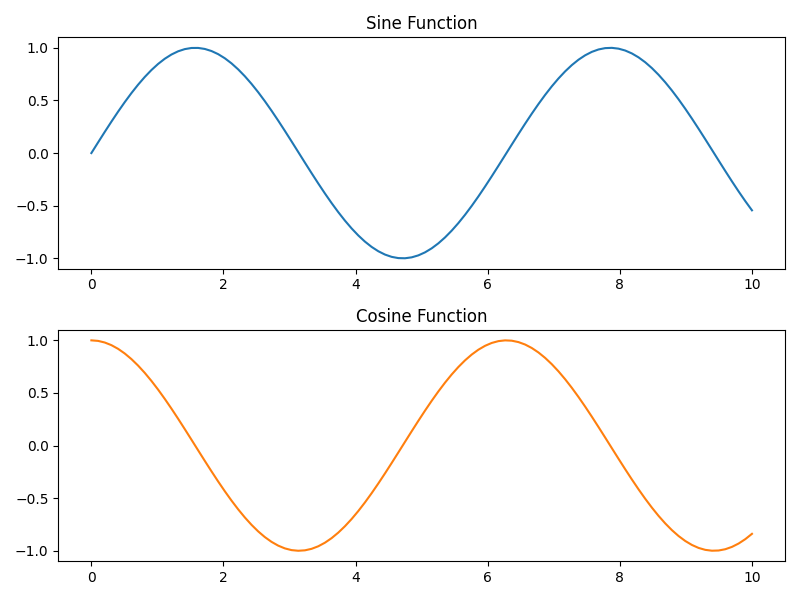
\includegraphics[width=0.8\textwidth]{images/plt/Figure_4.png}
\end{figure}

\subsection{风格和导出}

Matplotlib支持多种风格,可以通过\texttt{plt.style.use}函数来设置风格。例如,我们可以使用\texttt{science}和\texttt{ieee}风格来绘制图形,使得图形符合IEEE论文的格式要求:
\begin{lstlisting}[language=python]
plt.style.use(['science', 'ieee'])  # 需安装 SciencePlots
\end{lstlisting}
当然,如使用该风格,则默认需要LaTeX来渲染文本,而这是非常缓慢的。因此可以在该列表中添加\texttt{no-latex}选项,以禁用LaTeX渲染:
\begin{lstlisting}[language=python]
plt.style.use(['science', 'ieee', 'no-latex'])  # 需安装 SciencePlots
\end{lstlisting}

\begin{figure}[htbp]
    \centering
    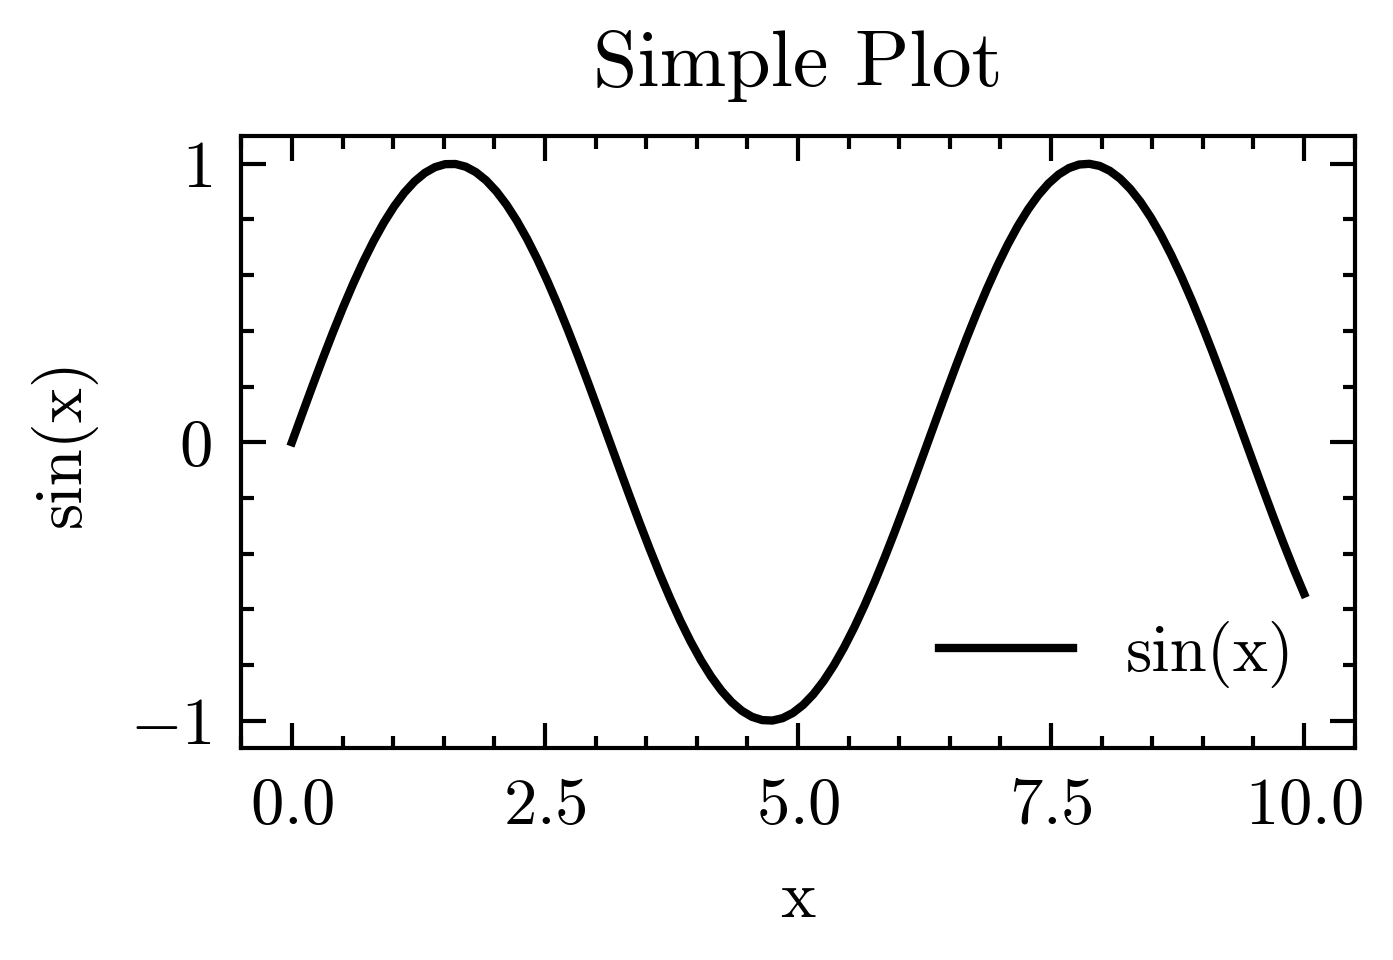
\includegraphics[width=0.8\textwidth]{images/plt/Figure_5.png}
    \caption{使用SciencePlots风格绘制的图形}
\end{figure}

此外,我们还可以将图形导出为各种格式,如PNG等:
\begin{lstlisting}[language=python]
plt.savefig('figure.svg')   # 矢量图
plt.savefig('figure.png', dpi=600, transparent=True) # PNG图    
\end{lstlisting}

\subsection{常见坑与提示}

\begin{itemize}
    \item 中文字体乱码:提前设置rcParams,或者使用\texttt{matplotlib.font\_manager}来设置中文字体。
    \begin{lstlisting}[language=python]
import matplotlib.pyplot as plt
plt.rcParams['font.sans-serif'] = ['SimHei']  # 设置中文字体
plt.rcParams['axes.unicode_minus'] = False  # 解决负号显示为方块的问题
    \end{lstlisting}
    \item 在Jupiter中不显示:使用\texttt{\%matplotlib inline}命令来确保图形在Jupyter Notebook中显示。
    \item 颜色过多:使用\texttt{tab:}前缀来使用Matplotlib内置的颜色表,避免颜色过多导致的混乱。
    \item 图例相互遮挡:使用\texttt{bbox\_to\_anchor}参数来调整图例的位置,或者\texttt{plt.legend(loc='best')}自动解决图例位置问题。
\end{itemize}

除此之外,Matplotlib还有许多其他的功能,如动画、3D绘图等,这些内容同学们可以在\href{https://matplotlib.org/stable/gallery/index.html}{Matplotlib官方示例}中找到。

\section{SymPy:符号计算高级计算器}

\begin{flushright}
    \emph{建议本节阅读者有一定的高等数学基础。}
\end{flushright}

SymPy是一个用于符号计算的Python库。符号计算是指对数学表达式进行符号操作,而不是数值计算;或者说,\textbf{求解析解而不是数值解}。SymPy可以用于求解方程、积分、微分、矩阵运算等多种数学操作。它的语法类似于Mathematica和Maple,但使用Python语言编写,因此更易于学习和使用。

在使用该库之前,我们尽量在文件的靠前位置写下这一行:\texttt{init\_printing(use\_unicode=True)},这样可以让SymPy的输出更加美观。

\subsection{基本数据类型}
SymPy的基本数据类型有三个:符号、表达式、等号。符号是SymPy的核心数据类型,用于表示数学符号,如变量、常数等。表达式是由符号和运算符组成的数学表达式,可以进行各种数学操作。等号用于表示等式关系。
\begin{lstlisting}[language=python]
    x, y = symbols('x y', real=True)  # 定义符号变量 x 和 y
    expr = x**2 + y**2  # 定义表达式
    line = Eq(y, 3*x + 2) # 定义等式
    print(expr)  # 输出表达式
\end{lstlisting}
上述代码定义了两个符号变量x和y,并定义了一个表达式$x^2 + y^2$和一个等式$y = 3x + 2$。SymPy的符号计算可以对这些符号进行各种操作,如求导、积分、化简等。

比方说:
\begin{lstlisting}
    expr = (x+1)*(x-2)-(x**2-2)
    simplify(expr)  # 化简表达式, 得到-x
    expand((x+1)**5)  # 展开多项式
    factor(x**3+1)  # 因式分解
    limit(expr, x, 0)  # 求expr在 x=0 处的极限
    diff(expr, x)  # 对 expr 求一次导数
    integrate(expr, x)  # 对 expr 求不定积分
    integrate(expr, (x, 0, 1))  # 对 expr 求定积分
    series(expr, x, 0, 5)  # 求泰勒级数展开,最高项次数为不超过4
    series(expr, x, 0, 5).removeO()  # 去掉高阶项
    solve(x**4-1, x)  # 求解等式x**4-1=0的解
    solve(a*x**2+b*x+c, x)  # 求解二次方程ax^2+bx+c=0的解,带着参数也能算
    nonlinsolve([x**2+y**2-1, x-y], (x, y))  # 求解非线性方程组
\end{lstlisting}

多元函数也可以使用上述方法来求导和积分,这里就不写了。需要注意的是,这里的求导数都是\textbf{偏导数}。一个非常有趣的事情是:在该库中,使用\texttt{-oo}和\texttt{oo}来表示负无穷和正无穷,而不是使用\texttt{float('inf')}。(疑似有些过于符号化了)

\subsection{矩阵和线性代数}
SymPy还提供了矩阵和线性代数的功能,可以进行矩阵运算、求逆、求特征值等操作。SymPy的矩阵是一个二维数组,可以进行各种矩阵运算,如加法、乘法、转置等。
\begin{lstlisting}[language=python]
    A = Matrix([[1, 2], [3, 4]])  # 定义一个矩阵
    b = Matrix([x, y])  # 定义一个列向量

    A.det()  # 求矩阵的行列式
    A.inv()  # 求矩阵的逆
    A.eigenvals()  # 求矩阵的特征值

    linsolve((A, b), [x, y])  # 求解线性方程组 Ax = b

    P, D = A.diagonalize()  # 对矩阵对角化,P为特征向量矩阵,D为对角矩阵
\end{lstlisting}

\subsection{输出、可视化}
在Jupiter里一行搞定输出,贴出来的字符串直接粘到论文里就能编译:
\begin{lstlisting}
    latex(Integral(exp(-x**2), (x, 0, oo)))
\end{lstlisting}

如果需要将表达式可视化,可以使用SymPy的\texttt{plot}函数来绘制函数图像:
\begin{lstlisting}[language=python]
    plot(sin(x)/x, (x, -10, 10))
\end{lstlisting}

\subsection{常见坑}
\begin{itemize}
    \item 符号爆炸:符号计算缓慢是正常现象,表达式也会越来越大。必要的时候,simplify、expand、factor等函数可以帮助我们化简表达式。
    \item 算错:这是常规现象,符号计算可能出现算错是不可避免的。我们可以快速使用数值验证结果的正确性。
    \item 并行:Sympy不能并行,但是可以拆任务并行计算(如multiprocessing)。
\end{itemize}

祝愿玩得开心,下次计算不用抄公式抄到手软!

\section{小练:抛体运动}

我们可以通过这个小项目来玩上述库,深化一下对它们的理解。当然,仅凭以上讲过的内容并不能很好地完成这些项目,同学们需要自己去查阅相关文档和资料,才能更好地完成这些小项目。

抛体运动是一个经典的物理问题。我们在高中阶段已经对该问题进行了深入的讨论和学习,但是并没有考虑诸如空气阻力等因素。现在,我们考虑空气阻力的影响,并使用相关的库来模拟抛体运动的轨迹。

思考:
\begin{itemize}
    \item 怎么计算轨迹?要数值解还是解析解?
    \item 怎么画图?画静态图还是动态图?
    \item 怎么考虑空气阻力?是线性还是非线性?
\end{itemize}

欢迎同学们踊跃思考,做出更好玩的demo!

\end{document}